\documentclass[12pt, titlepage]{article}

\usepackage{booktabs}
\usepackage{tabularx}
\usepackage{hyperref}
\usepackage{float}
\usepackage{fullpage}
\usepackage[round]{natbib}
\usepackage{multirow}
\usepackage{booktabs}
\usepackage{tabularx}
\usepackage{graphicx}
\usepackage{float}
\usepackage{hyperref}
\usepackage{xcolor}
\restylefloat{table}
\hypersetup{
    colorlinks,
    citecolor=black,
    filecolor=black,
    linkcolor=red,
    urlcolor=blue
}
\usepackage[round]{natbib}

\title{SE 3XA3: Test Report\\Othello}

\author{Team \#2, JSM Corporation
		\\ Jinesh Patel and patelj60
		\\ Mohammed Mirajkar  and mirajkam
		\\ Sankar Renganathan and renganas
}

\date{\today}

%\input{../Comments}

\begin{document}

\maketitle

\pagenumbering{roman}
\tableofcontents
\listoftables
\listoffigures

\begin{table}[bp]
	\caption{\bf Revision History}
	\begin{tabularx}{\textwidth}{p{3cm}p{2cm}X}
		\toprule {\bf Date} & {\bf Version} & {\bf Notes}  \\
		\midrule
		2018-12-05          & 1.0           & Evaluations  \\
		2018-12-05          & 1.1           & Test Results \\
		2018-12-05          & 1.2           & Comparisons  \\
		\bottomrule
	\end{tabularx}
\end{table}

\newpage

\pagenumbering{arabic}

This document will go over the testing procedures and results that have been used and observed throughout the development process for Othello.

\section{Functional Requirements Evaluation}
\begin{enumerate}
	\item Test Name: FR-UserValidity\\
	      Results: All green cells representing the moves the user can make is valid according to the rules of Othello
	\item Test Name: FR-AIValidity\\
	      Results: All green cells representing the moves the AI can make is valid according to the rules of Othello
	\item Test Name: FR-Invalid\\
	      Results: Board state does not change when use makes invalid move
	\item Test Name: FR-Save\\
	      Results: Current state of board is saved in local storage after user clicks save button
	\item Test Name: FR-Load\\
	      Results: State of board in local storage is retrieved after user clicks load button
	\item Test Name: FR-Undo\\
	      Results: State of board is restored to the most recent state of the board on the history stack
	\item Test Name: FR-Reset\\
	      Results: State of board is 2 black and white pieces in the middle
	\item Test Name: FR-Score\\
	      Results: The white score corresponds to number of white pieces on board while black score corresponds to number of black pieces on board
	\item Test Name: FR-Victory\\
	      Results: Victory screen displays a win message if user has a higher score than AI, lose message if user has a lower score than AI, and a tie message if user has the same score as AI
\end{enumerate}

\section{Nonfunctional Requirements Evaluation}

\subsection{Usability}
Method of Testing: A group of 8 people comprising of a group of 5 McMaster students from different faculties, 1 student in Grade 11, 1 student in Grade 6 and one student in Grade 1 were surveyed while playing JSM corporation's implementation of Othello
\begin{enumerate}
	\item Test Name: NFR-Interface\\
	      Results: All participants were able to navigate through the main screen and understand the functionalities of the button with an average of 2.5 minutes. The maximum time it took for an individual to get comfortable with the interface was 3 minutes and 10 seconds which is significantly lower than the expected time it would take to get used to the interface which was 5 minutes.
	\item Test Name: NFR-Rules\\
	      Results: All participants were able to understand the rules of the game within a minute which was lower than the expected time of 3 minutes.
\end{enumerate}

\subsection{Performance}
\begin{enumerate}
	\item Test Name: NFR-AITime\\
	      Method: In-built timer is used to record the execution time for the AI to make a move\\
	      Results: AI makes moves in under 1 second
	\item Test Name: NFR-MoveTime\\
	      Method: In-built timer is used to record the execution time for the board state to change after the user selects a move\\
	      Results: User's selected move is displayed in board in under a second
	\item Test Name: NFR-AnimTime\\
	      Method: In-built timer is used to record the time it takes for an animation to complete\\
	      Results: Animations/transitions displayed on interface are completed in under 2 seconds
\end{enumerate}

\subsection{Operations and Environment}
\begin{enumerate}
	\item Test Name: NFR-IO\\
	      Method: Othello was played using a logitech mouse, Razer gaming mouse, and an HP Pavillion trackpad\\
	      Results: Othello is compatible with all mouse types listed above
	\item Test Name: NFR-Browser\\
	      Method: Othello was played using FireFox, Chrome, Edge, Safari and Opera\\
	      Results: Othello runs on all browsers listed above
\end{enumerate}


\subsection{Maintainability}
\begin{enumerate}
	\item Test Name: NFR-Git\\
	      Method: McMaster software student was asked to navigate through git repository and find certain file\\
	      Results: Student was able to find AI module under 10 seconds, Board module in under 10 and was able to identify the main purpose of the module in under 3 minutes
\end{enumerate}

\section{Comparison to Existing Implementation}

This section will not be appropriate for every project.

\section{Unit Testing}
\label{sec:ut}
\hypertarget{sec:ccm}{}

Unit Testing is performed on modules Board, History and AI as these are the fundamental parts of the software that don't have high integration and high dependency with the other modules. The strategy for unit testing was to test all the module functions that are avaialable to the external interface with as many possibilities of input to the functions that can test the greatest amount of equivalence classes. The Unit testing results can be found in the resulting generated file under the src folder, called 'test-report.html'. Coverage of the unit tests are found under \hyperref[sec:ccm]{Code Coverage Metrics}.

\subsection {History}
\subsubsection {Testing Constructor}
\begin{enumerate}
	\item Test default constructor. \begin{itemize}
		      \item Initial: No initial state.
		      \item Input: Create a history instance with no parameters.
		      \item Expected Output: The history instance has an empty timeline.
	      \end{itemize}
		\item Test constructor with predefined previous state.\begin{itemize}
				\item Initial: No initial state.
				\item Input: Create a history instance with the predefined previous states.
				\item Expected Output: The history instance timeline has the predefined previous states in the same order.
			\end{itemize}
\end{enumerate}

\subsubsection {Testing canUndo()}
\begin{enumerate}
	\item Test canUndo. \begin{itemize}
		      \item Initial: A history instance filled with some previous states and another instance with no previous states.
		      \item Input: Call the canUndo function with no parameters.
		      \item Expected Output: \texttt{true} when there are previous states and \texttt{false} when there aren't.
	      \end{itemize}
\end{enumerate}

\subsubsection {Testing undo()}
\begin{enumerate}
	\item Test undo. \begin{itemize}
		      \item Initial: A history instance filled with some previous states.
		      \item Input: Call the undo function with no parameters.
		      \item Expected Output: The previous state of the object.
	      \end{itemize}
	\item Test errors. \begin{itemize}
		      \item Initial: A history instance with no previous states.
		      \item Input: Call the undo function with no parameters.
		      \item Expected Output: The functions throws a \texttt{CannotUndo} error.
	      \end{itemize}
\end{enumerate}

\subsubsection {Testing reset()}
\begin{enumerate}
	\item Test reset. \begin{itemize}
		      \item Initial: A history instance filled with some previous states.
		      \item Input: Call the reset function with no parameters.
		      \item Expected Output: The history timeline becomes empty.
	      \end{itemize}
\end{enumerate}

\subsubsection {Testing push(data)}
\begin{enumerate}
	\item Test push. \begin{itemize}
		      \item Initial: A history instance with no previous states.
		      \item Input: Call the push function with states of an object.
		      \item Expected Output: The history timeline contains all those states in the order they were pushed.
	      \end{itemize}
\end{enumerate}

\subsubsection {Testing time()}
\begin{enumerate}
	\item Test time. \begin{itemize}
		      \item Initial: A history instance with a defined amount of previous states.
		      \item Input: Call the time function with no parameters.
		      \item Expected Output: The number of previous states.
	      \end{itemize}
\end{enumerate}

\subsubsection {Testing peek(i)}
\begin{enumerate}
	\item Test peek. \begin{itemize}
		      \item Initial: A history instance with some previous states.
		      \item Input: Call the peek function with an integer within the time amount of history.
		      \item Expected Output: The state of the object at the specified time.
	      \end{itemize}
\end{enumerate}

\subsubsection {Testing timeline()}
\begin{enumerate}
	\item Test timeline. \begin{itemize}
		      \item Initial: A history instance with some previous states.
		      \item Input: Call the timeline function with no parameters.
		      \item Expected Output: The previous states all in the correct order.
	      \end{itemize}
\end{enumerate}

\subsection{AI}
\subsubsection {Testing pick function for different difficulties}
\begin{enumerate}
	\item Test pick function to see if it acts the same as the sub pick function at difficulty 0. \begin{itemize}
		      \item Initial: An ai instance with difficulty set to 0.
		      \item Input: Call the pick function with no parameters.
		      \item Expected Output: A valid move and the pickMoveRandom function has been called with the return value of pick the same as the one from pickMoveRandom.
	      \end{itemize}
	\item Test pick function to see if it acts the same as the sub pick function at difficulty 1. \begin{itemize}
		      \item Initial: An ai instance with difficulty set to 1.
		      \item Input: Call the pick function with no parameters.
		      \item Expected Output: A valid move and the pickMoveAverage function has been called with the return value of pick the same as the one from pickMoveAverage.
	      \end{itemize}
	\item Test pick function to see if it acts the same as the sub pick function at difficulty 2. \begin{itemize}
		      \item Initial: An ai instance with difficulty set to 2.
		      \item Input: Call the pick function with no parameters.
		      \item Expected Output: A valid move and the pickMoveSmart function has been called with the return value of pick the same as the one from pickMoveSmart.
	      \end{itemize}
\end{enumerate}

\subsubsection {Testing pickMoveRandom}
\begin{enumerate}
	\item Test if it returns one of the moves given. \begin{itemize}
		      \item Initial: An ai instance with difficulty set to 0.
		      \item Input: Call the pickMoveRandom function with a set of possible moves.
		      \item Expected Output: The returned move is one of the possible moves.
	      \end{itemize}
	\item Test function errors. \begin{itemize}
		      \item Initial: An ai instance with difficulty set to 0.
		      \item Input: Call the pickMoveRandom function with no moves.
		      \item Expected Output: Throws an error called \texttt{NoMoves}.
	      \end{itemize}
\end{enumerate}

\subsubsection {Testing pickMoveAverage}
\begin{enumerate}
	\item Test if it returns a valid move. \begin{itemize}
		      \item Initial: An ai instance with difficulty set to 1.
		      \item Input: Call the pickMoveAverage function with a board state.
		      \item Expected Output: The returned move is a valid move according to the board state.
	      \end{itemize}
	\item Test the preferencing. \begin{itemize}
		      \item Initial: An ai instance with difficulty set to 1.
		      \item Input: Call the pickMoveAverage function with certain board states.
		      \item Expected Output: Returns the prefered move that was computed by the tester.
	      \end{itemize}
	\item Test for no moves. \begin{itemize}
		      \item Initial: An ai instance with difficulty set to 1.
		      \item Input: Call the pickMoveAverage function with a board state that does not allow any moves.
		      \item Expected Output: Returns \texttt{null}.
	      \end{itemize}
\end{enumerate}

\subsubsection {Testing pickMoveSmart}
\begin{enumerate}
	\item Test if it returns a valid move. \begin{itemize}
		      \item Initial: An ai instance with difficulty set to 2.
		      \item Input: Call the pickMoveSmart function with a board state.
		      \item Expected Output: The returned move is a valid move according to the board state and corresponds to the move returned by the minimax algorithm.
	      \end{itemize}
	\item Test the algorithm. \begin{itemize}
		      \item Initial: An ai instance with difficulty set to 2.
		      \item Input: Call the pickMoveSmart function with certain board states.
		      \item Expected Output: returns a move that is computed by the minimax algorithm
	      \end{itemize}
	\item Test for no moves. \begin{itemize}
		      \item Initial: An ai instance with difficulty set to 2.
		      \item Input: Call the pickMoveSmart function with a board state that does not allow any moves.
		      \item Expected Output: Returns \texttt{null}.
	      \end{itemize}
\end{enumerate}

\subsubsection {Testing getDifficulty}
\begin{enumerate}
	\item Test function. \begin{itemize}
		      \item Initial: An ai instance set to a certain difficulty.
		      \item Input: A call to the getDifficulty function.
		      \item Expected Output: The returned difficulty is the same as the set difficulty.
	      \end{itemize}
\end{enumerate}

\subsubsection {Testing setDifficulty}
\begin{enumerate}
	\item Test function. \begin{itemize}
		      \item Initial: An ai instance set to a certain difficulty.
		      \item Input: A call to the setDifficulty function with a different difficulty.
		      \item Expected Output: The difficulty of the ai instance is updated.
	      \end{itemize}
\end{enumerate}

\subsection {Board}
\subsubsection {Testing Constructor}
\begin{enumerate}
	\item Test default constructor. \begin{itemize}
		      \item Initial: None
		      \item Input: Size
		      \item Expected Output: Default 8x8 board
	      \end{itemize}
	\item Test constructor with specific board state.\begin{itemize}
		      \item Initial: None
		      \item Input: Size and State of board
		      \item Expected Output: 8x8 board with the predefined state
	      \end{itemize}
	\item Test default constructor with invalid size. \begin{itemize}
		      \item Initial: None
		      \item Input: Invalid size
		      \item Expected Output: Exception for invalid size
	      \end{itemize}
	\item Test constructor with invalid state.\begin{itemize}
		      \item Initial: None
		      \item Input: Invalid state
		      \item Expected Output: Exception for invalid state
	      \end{itemize}
\end{enumerate}

\subsubsection {getBoardSize Test}
\begin{enumerate}
	\item Test getBoardSize(). \begin{itemize}
		      \item Initial: Current state of board.
		      \item Input: None
		      \item Expected Output: The current size of the board
	      \end{itemize}
\end{enumerate}

\subsubsection {isCellInBoard Test}
\begin{enumerate}
	\item Test isCellInBoard \begin{itemize}
		      \item Initial: No initial state.
		      \item Input: The i$^{th}$ row and j$^{th}$ column of the board
		      \item Expected Output: \texttt{true} if given coordinates are in the board, \texttt{false} if not
	      \end{itemize}
\end{enumerate}

\subsubsection {Testing isCellValue}
\begin{enumerate}
	\item Test isCellValue \begin{itemize}
		      \item Initial: Current board state
		      \item Input: The i$^{th}$ row and j$^{th}$ column of board as well as a cell value
		      \item Expected Output: \texttt{true} if cell value matches the value in the given cell coordinates, \texttt{false} otherwise
	      \end{itemize}
	\item Test isCellValue Error \begin{itemize}
		      \item Initial: Current board state
		      \item Input: The i$^{th}$ row and j$^{th}$ column of board that is invalid as well as a cell value
		      \item Expected Output: A thrown error indicating invalid cell location or value.
	      \end{itemize}
\end{enumerate}

\subsubsection {Testing Valid}
\begin{enumerate}
	\item Test Valid \begin{itemize}
		      \item Initial: Current board state
		      \item Input: The i$^{th}$ row and j$^{th}$ column of board as well as which play's turn it currently is
		      \item Expected Output: True if the cell is valid as well as the possible score for that cell
	      \end{itemize}
	\item Test Valid Error \begin{itemize}
		      \item Initial: Current board state
		      \item Input: The i$^{th}$ row and j$^{th}$ column of board that contains an invalid value as well as which play's turn it currently is
		      \item Expected Output: A thrown error indicating invalid cell location or value.
	      \end{itemize}
\end{enumerate}

\subsubsection {Testing Move}
\begin{enumerate}
	\item Test Move \begin{itemize}
		      \item Initial: Current board state
		      \item Input: The i$^{th}$ row and j$^{th}$ column of board as well as which play's turn it currently is
		      \item Expected Output: None (Function does not return anything. Output is seen in UI. )
	      \end{itemize}
	\item Test Move Error \begin{itemize}
		      \item Initial: Current board state
		      \item Input: The i$^{th}$ row and j$^{th}$ column of board that is invalid in terms of the rules as well as which player's turn it currently is
		      \item Expected Output: Error thrown indicating an invalid cell location or invalid move.
	      \end{itemize}
\end{enumerate}

\subsubsection{Testing getCellValue}
\begin{enumerate}
	\item Test setCell \begin{itemize}
		      \item Initial: Current board state
		      \item Input: The i$^{th}$ row and j$^{th}$ of board as well and the value of the piece in that position.
		      \item Expected Output: None (Function does not return anything as it is a mutator. Verification is done by getting the value of the boards property. In whch case, the state attribute of board must have value v at index(x,y).
	      \end{itemize}
	\item Test setCell Error \begin{itemize}
		      \item Initial: Current board state
		      \item Input: The i$^{th}$ row and j$^{th}$ column of board that is invalid in terms of the board size
		      \item Expected Output: Exception thrown indicating an invalid value or invalid coordinates
	      \end{itemize}
\end{enumerate}

\subsubsection{Testing getCellValue}
\begin{enumerate}
	\item Test getCell \begin{itemize}
		      \item Initial: Current board state
		      \item Input: The i$^{th}$ row and j$^{th}$ column of board to get cell value from.
		      \item Expected Output: The value of the piece currently in that cell
	      \end{itemize}
	\item Test getCell Error \begin{itemize}
		      \item Initial: Current board state
		      \item Input: The i$^{th}$ row and j$^{th}$ column of board that is invalid in terms of the board size
		      \item Expected Output: Exception thrown indicating invalid coordinates
	      \end{itemize}
\end{enumerate}


\subsubsection{Testing getCount}
\begin{enumerate}
	\item Test getCount \begin{itemize}
		      \item Initial: Current board state
		      \item Input: valid piece type/value
		      \item Expected Output: The number of pieces of value v on the board.
	      \end{itemize}
	\item Test getCount Error\begin{itemize}
		      \item Initial: Current board state
		      \item Input: invalid piecetype/value
		      \item Expected Output: Exception thrown indicating invalid value.
	      \end{itemize}
\end{enumerate}


\subsubsection{Testing setState}
\begin{enumerate}
	\item Test setState \begin{itemize}
		      \item Initial: Current board state
		      \item Input: any valid board state
		      \item Expected Output: None (Function does not return anything as it is a mutator). Verification is done by getting the value of the board objects state attirbute and comparing it to another board object with the same state.
	      \end{itemize}
	\item Test setState Error\begin{itemize}
		      \item Initial: Current board state
		      \item Input: invalid board state
		      \item Expected Output: Exception thrown indicating come form of invalid board state.
	      \end{itemize}
\end{enumerate}


\subsubsection{Testing findValidMoves}
\begin{enumerate}
	\item Test findValidMoves \begin{itemize}
		      \item Initial: Current board state
		      \item Input:  the player's piece color whose turn it currently is
		      \item Expected Output: All valid moves for the player whose turn it is currently .
	      \end{itemize}
	\item Test findValidMoves Error \begin{itemize}
		      \item Initial: Current board state
		      \item Input: invalid player designator
		      \item Expected Output: Exception thrown indicating no such color for player exists.
	      \end{itemize}
\end{enumerate}

\subsubsection{Testing ignore}
\begin{enumerate}
	\item Test ignore \begin{itemize}
		      \item Initial: Current board state
		      \item Input: A callback function
		      \item Expected Output: The callback function should be called 0 times.
	      \end{itemize}
\end{enumerate}

\subsubsection{Testing notify}
\begin{enumerate}
	\item Test notify \begin{itemize}
		      \item Initial: Current board state
		      \item Input: Call notify
		      \item Expected Output: The set of callback functions has been called.
	      \end{itemize}
\end{enumerate}

\subsubsection{Testing listen}
\begin{enumerate}
	\item Test listen \begin{itemize}
		      \item Initial: Current board state
		      \item Input: A callback function.
		      \item Expected Output: The callback function should be called 1 or more times.
	      \end{itemize}
\end{enumerate}

\section{Changes Due to Testing}

\subsection{Board Module}
The valid function was returing the wrong potential score which was changed such to return the correct amount. 

\subsection{AI Module}
The minimax algorithm for the hard AI was changed to incorporate a region-based thinking heuristic that we use in our medium AI. The change was mandated after it was discovered during testing that the hard AI felt easier to beat compared to the medium AI. After incroporating the region-based algorithm, the feedback from testers all marked the AI as being much harder to beat. 

\subsection{History Module}
No changes were made to the history module.

\section{Automated Testing}
\hypertarget{sec:ccm}{}

Automated Testing is performed using Jest (requires Node.js and npm to be installed) in the Visual Studio Code IDE. The report is generated through Jest-HTML-Reporter plugin for Jest. Automated testing was best suited towards unit testing as stubs and drivers are very easily created for the particular modules and functions that were tested through unit testing. It was best to test the integrated software and UI elements with manual testing as it was more time efficient to do so for the schedule of this project as writing the test cases for UI has a large learning curve. The results of the automated testing are given in the \hyperref[sec:ut]{Unit Testing} section. You can find the coverage report of these tests in the \hyperref[sec:ccm]{Code Coverage Metrics} section.

To run automated tests, the best way is to use a Unix based terminal with the cloned repository and from the src directory run the command \texttt{./node\char`_modules/jest/bin/jest.js --coverage}. This should output the testing results as well as the coverage in the terminal and also generate 'test-report.html' for the test results as well as 'index.html' under a generated folder named 'coverage/lcov-report'.

\newpage
\section{Trace to Requirements}
\begin{table}[H]
	\caption{Trace Between Tests and Requirements}
	\begin{tabularx}{\textwidth}{ll}
		\toprule
		Test            & Requirements                          \\
		\midrule
		\multicolumn{2}{c}{Functional Requirements Testing}     \\
		\midrule
		FR-Victory      & FR2, FR12                             \\
		FR-UserValidity & FR5, FR6                              \\
		FR-AIValidity   & FR4, FR5                              \\
		FR-Invalid      & FR5, FR7                              \\
		FR-Save         & FR8, FR11                             \\
		FR-Load         & FR11,  FR12                           \\
		FR-Undo         & FR10                                  \\
		FR-Score        & FR5                                   \\
		FR-Reset        & FR3, FR9                              \\

		\midrule
		\multicolumn{2}{c}{Non-functional Requirements Testing} \\
		\midrule
		NFR-Interface   & NF1, NF2, NF3, NF4, NF5,NF6, NF14     \\
		NFR-Rules       & NF5, NF6                              \\
		NFR-AITime      & NF7                                   \\
		NFR-MoveTime    & NF8                                   \\
		NFR-AnimTime    & NF9                                   \\
		NFR-IO          & NF10                                  \\
		NFR-Browser     & NF11                                  \\
		NFR-Git         & NF12, NF15                            \\
		\bottomrule
	\end{tabularx}
\end{table}

\section{Trace to Modules}
\begin{table}[H]
	\begin{tabularx}{\textwidth}{ll}
		\toprule
		Test            & Requirements                          \\
		\midrule
		FR-Victory      & M3, M4                                \\
		FR-UserValidity & M2, M4                                \\
		FR-AIValidity   & M2, M4, M6                            \\
		FR-Invalid      & M2, M4                                \\
		FR-Save         & M1,M5                                 \\
		FR-Load         & M1,M5                                 \\
		FR-Undo         & M1,M5                                 \\
		FR-Score        & M1, M2                                \\
		FR-Reset        & M1, M5                                \\
		\midrule
		\multicolumn{2}{c}{Non-functional Requirements Testing} \\
		\midrule
		NFR-Interface   & M1                                    \\
		NFR-Rules       & M1                                    \\
		NFR-AITime      & M1, M6                                \\
		NFR-MoveTime    & M1                                    \\
		NFR-AnimTime    & NF9                                   \\
		NFR-IO          & N/A                                   \\
		NFR-Browser     & N/A                                   \\
		NFR-Git         & N/A                                   \\
		\bottomrule
	\end{tabularx}
	\caption{Trace Between Tets and Modules}
\end{table}


\section{Code Coverage Metrics}
\label{sec:ccm}
Our group has made tests that cover 100\% of all statements in the tested modules which consist of the AI class, the Board class, and the History class respectively. This number has been retrieved from the our tests  using the Jest testing application. A picture has been provided below to show that our tests truly cover 100\% of the tested modules. Additionally, one can also refer to the coverage document which is in the location 'Coverage/Lcov Report'. 

\begin{figure}[H]
\centering
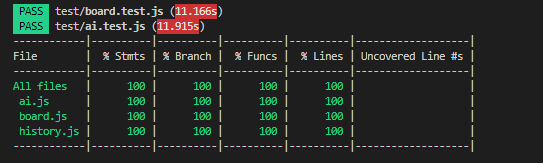
\includegraphics[width=0.8\textwidth]{CodeCoverage.png}
\caption{Code Coverage Metrics}
\label{FigUH}
\end{figure}

\bibliographystyle{plainnat}

\bibliography{SRS}

\end{document}